\section{Dynamic Programming}
\subsection{Weighted Interval Scheduling}
\emph{The idea:} Sort by finish time and select: \\
\begin{equation*}
    \text{OPT}(j) = 
    \begin{cases}
        \text{max}(v[j]) + \text{OPT}(p[j]) \\
        \text{OPT}(j-1)
    \end{cases}
\end{equation*}
Either you take job $j$, and skip conflicts, or don't take
it. The algorithm runs in $O(n \log n)$ time, where $n$ is the number of jobs.

\begin{figure}[h]
\centering
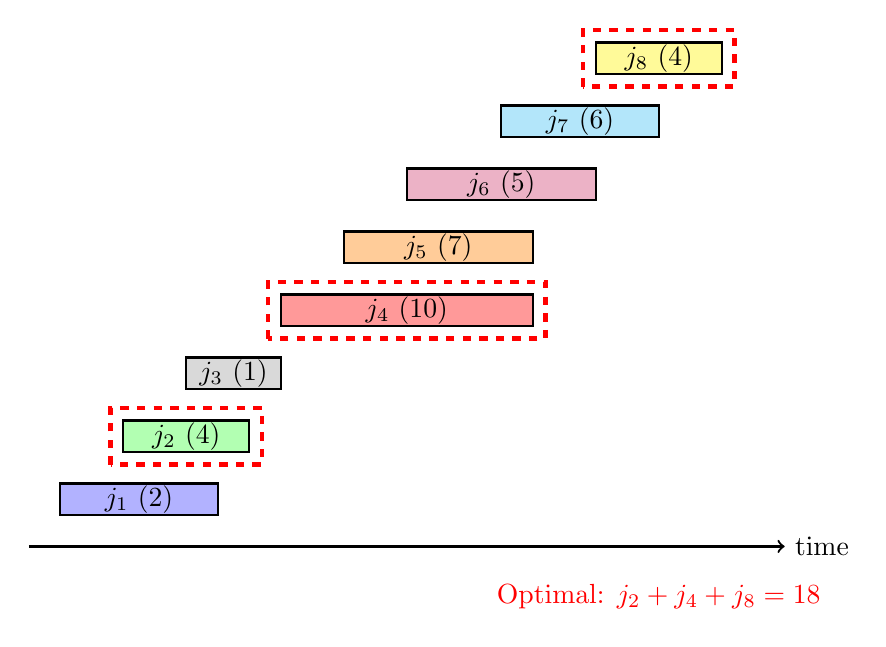
\begin{tikzpicture}[scale=0.8]
    % Time axis
    \draw[->,thick] (0,0) -- (12,0) node[right] {time};
    
    % Job 1: v=2
    \draw[fill=blue!30,draw=black,thick] (0.5,0.5) rectangle (3,1) node[pos=0.5] {$j_1$ (2)};
    
    % Job 2: v=4
    \draw[fill=green!30,draw=black,thick] (1.5,1.5) rectangle (3.5,2) node[pos=0.5] {$j_2$ (4)};
    
    % Job 3: v=1
    \draw[fill=gray!30,draw=black,thick] (2.5,2.5) rectangle (4,3) node[pos=0.5] {$j_3$ (1)};
    
    % Job 4: v=10
    \draw[fill=red!40,draw=black,thick] (4,3.5) rectangle (8,4) node[pos=0.5] {$j_4$ (10)};
    
    % Job 5: v=7
    \draw[fill=orange!40,draw=black,thick] (5,4.5) rectangle (8,5) node[pos=0.5] {$j_5$ (7)};
    
    % Job 6: v=5
    \draw[fill=purple!30,draw=black,thick] (6,5.5) rectangle (9,6) node[pos=0.5] {$j_6$ (5)};
    
    % Job 7: v=6
    \draw[fill=cyan!30,draw=black,thick] (7.5,6.5) rectangle (10,7) node[pos=0.5] {$j_7$ (6)};
    
    % Job 8: v=4
    \draw[fill=yellow!40,draw=black,thick] (9,7.5) rectangle (11,8) node[pos=0.5] {$j_8$ (4)};
    
    % Highlight optimal solution
    \draw[red,ultra thick,dashed] (1.3,1.3) rectangle (3.7,2.2);
    \draw[red,ultra thick,dashed] (3.8,3.3) rectangle (8.2,4.2);
    \draw[red,ultra thick,dashed] (8.8,7.3) rectangle (11.2,8.2);
    
    \node[red] at (10,-0.8) {Optimal: $j_2 + j_4 + j_8 = 18$};
\end{tikzpicture}
\caption{Weighted Interval Scheduling Example: Jobs are sorted by finish time. The optimal solution selects non-overlapping jobs with maximum total value.}
\end{figure}


\subsection{Subset Sum}


\subsection{Knapsack}

\emph{The problem:} Fill a backpack with as many books as possible. \\
\begin{equation*}
    \text{OPT}(i,w) = 
    \begin{cases}
        \text{OPT}(i-1,w) \\
        v[i] + \text{OPT}(i-1, w-w[i])
    \end{cases}
\end{equation*}
The option is to take an item $i$ or not and the algorithm runs in $O(nW)$
time, where $n$ is the number of items and $W$ is knapsack capacity. The
algorithm creates a 2D table consisting of $n\times W$
